\subsection{Experimental setup}
\label{sec:setup}

\subsubsection{System}
\label{sec:system}

For our experiments, we use a server that has an x86-based 64-bit AMD EPYC-7742 processor. This processor has a clock frequency of 2.25 GHz and 512 GB of DDR4 system memory. Each core has an L1 cache of 4 MB, an L2 cache of 32 MB, and a shared L3 cache of 256 MB. The machine runs on Ubuntu 20.04. We use GCC 9.4 and OpenMP 5.0 \cite{openmp18}.


\subsubsection{Configuration}
\label{sec:configuration}

We use 32-bit unsigned integer for vertex ids, 32-bit floating point for edge weights, but use 64-bit floating point for hashtable values, total edge weight, modularity calculation, and all places where performing an aggregation/sum of floating point values. Unless mentioned otherwise, we execute all parallel implementations with a default of $64$ threads (to match the number of cores available on the system).

\begin{table}[hbtp]
  \centering
  \caption{List of $13$ graphs obtained SuiteSparse Matrix Collection \cite{suite19} (directed graphs are marked with $*$). Here, $|V|$ is the number of vertices, $|E|$ is the number of edges (after adding reverse edges), $D_{avg}$ is the average degree, and $|\Gamma|$ is the number of communities obtained using Louvain algorithm.\ignore{In the table, B refers to a billion, M refers to a million and K refers a thousand.}}
  \label{tab:dataset}
  \begin{tabular}{|c||c|c|c|c|}
    \toprule
    \textbf{Graph} &
    \textbf{\textbf{$|V|$}} &
    \textbf{\textbf{$|E|$}} &
    \textbf{\textbf{$D_{avg}$}} &
    \textbf{\textbf{$|\Gamma|$}} \\
    % \textbf{$1 - \Gamma_G$} \\
    \midrule
    \multicolumn{5}{|c|}{\textbf{Web Graphs (LAW)}} \\ \hline
    indochina-2004$^*$ & 7.41M & 341M & 41.0 & 4.24K \\ \hline  % & \num{4.7e-4} & 2.9 GB
    uk-2002$^*$ & 18.5M & 567M & 16.1 & 42.8K \\ \hline  % & \num{9.6e-5} & 16 GB
    arabic-2005$^*$ & 22.7M & 1.21B & 28.2 & 3.66K \\ \hline  % & \num{5.5e-4} & 11 GB
    uk-2005$^*$ & 39.5M & 1.73B & 23.7 & 20.8K \\ \hline  % & \num{9.6e-5} & 16 GB
    webbase-2001$^*$ & 118M & 1.89B & 8.6 & 2.76M \\ \hline  % & \num{7.3e-7} & 18 GB
    it-2004$^*$ & 41.3M & 2.19B & 27.9 & 5.28K \\ \hline  % & \num{3.8e-4} & 19 GB
    sk-2005$^*$ & 50.6M & 3.80B & 38.5 & 3.47K \\ \hline  % & \num{5.8e-4} & 33 GB
    \multicolumn{5}{|c|}{\textbf{Social Networks (SNAP)}} \\ \hline
    com-LiveJournal & 4.00M & 69.4M & 17.4 & 2.54K \\ \hline  % & \num{7.9e-4} & 480 MB
    com-Orkut & 3.07M & 234M & 76.2 & 29 \\ \hline  % & \num{6.7e-2} & 1.7 GB
    \multicolumn{5}{|c|}{\textbf{Road Networks (DIMACS10)}} \\ \hline
    asia\_osm & 12.0M & 25.4M & 2.1 & 2.38K \\ \hline  % & \num{8.4e-4} & 200 MB
    europe\_osm & 50.9M & 108M & 2.1 & 3.05K \\ \hline  % & \num{6.6e-4} & 910 MB
    \multicolumn{5}{|c|}{\textbf{Protein k-mer Graphs (GenBank)}} \\ \hline
    kmer\_A2a & 171M & 361M & 2.1 & 21.2K \\ \hline  % & \num{9.4e-5} & 3.2 GB
    kmer\_V1r & 214M & 465M & 2.2 & 6.17K \\ \hline  % & \num{3.2e-4} & 4.2 GB
  \bottomrule
  \end{tabular}
\end{table}
% We convert directed graphs (marked with $*$) to undirected by duplicating edges in the reverse direction, and set the weight of each edge to $1$. and $F_{size}$ is size of the \textit{MatrixMarket} file



\subsubsection{Reproducibility}
\label{sec:reproducibilty}

All our results are reproducible. The source code for the experiments reported in this paper along with necessary scripts for obtaining the datasets and compiling the software is available at \url{https://bit.ly/hipc23-174}. 


\subsubsection{Dataset}
\label{sec:dataset}

Table \ref{tab:dataset} shows the graphs we use in our experiments. All of them are obtained from the SuiteSparse Matrix Collection \cite{suite19}. The number of vertices in the graphs varies from $3.07$ to $214$ million, and the number of edges varies from $25.4$ million to $3.80$ billion. We ensure that all edges are undirected and weighted with a default weight of $1$.


\subsubsection{Batch generation}
\label{sec:batch-update}

We take a base graph from the dataset and generate a random batch update \cite{com-zarayeneh21} consisting of an equal mix of edge deletions and insertions \cite{com-chong13}, each with an edge weight of $1$. All batch updates are undirected, i.e., for every edge insertion $(i, j, w)$ in the batch update, the edge $(j, i, w)$ is also a part of the batch update. For simplicity, we generate these edges such that the selection of each vertex (as endpoint) is equally probable, and we do not add any new vertices to the graph. Testing with batches having other distributions is part of our future work.

\begin{figure*}[hbtp]
  \centering
  \subfigure[Results of each graph]{
    \label{fig:louvain--all}
    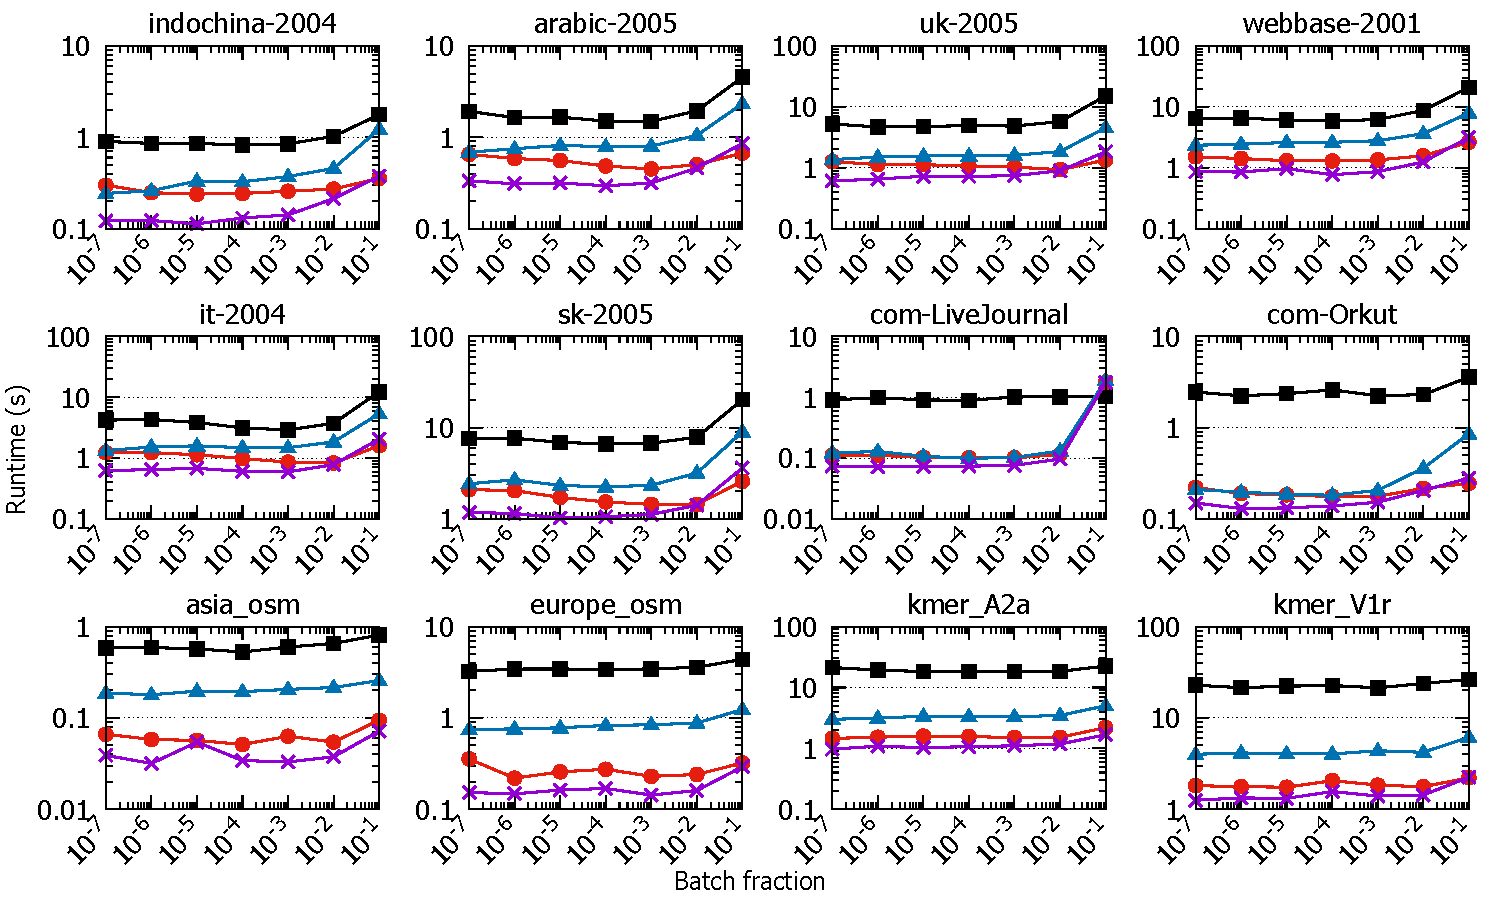
\includegraphics[width=0.58\linewidth]{out/louvain-all-fullx.pdf}
  }
  \subfigure[Overall result]{
    \label{fig:louvain--am}
    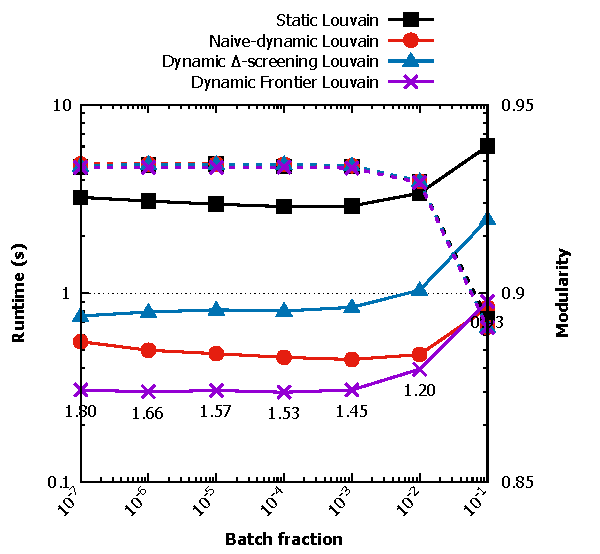
\includegraphics[width=0.38\linewidth]{out/louvain-am.pdf}
  } \\[-2ex]
  \caption{Time taken (solid lines), and modularity of communities obtained (dashed lines) along the right Y-axis, with \StaLou{}, \NaiLou{}, \DelLou{}, and \FroLou (Algorithm \ref{alg:louvain}) on batch updates of increasing size from $10^{-7} |E|$ to $0.1 |E|$. Note that both axes are logarithmic. Speedup of \FroLou{} with respect to \NaiLou{} is labeled.}
  \label{fig:louvain}
\end{figure*}


\paragraph{Adjusting batch size}

For all dynamic graph-based experiments, we modify the batch size as a fraction of the total number of edges in the original (undirected) graph from $10^{-7}$ to $0.1$ (i.e., $10^{-7}|E|$ to $0.1|E|$). For a billion-edge graph, this amounts to a batch size of $100$ to $100$ million edges. Keep in mind that dynamic graph algorithms are helpful for small batch sizes in interactive applications. For large batches, it is usually more efficient to run the static algorithm.

\paragraph{Minimizing measurement noise}

We employ $5$ distinct random batch updates for each batch size and report average across these runs in our experiments.


\subsubsection{Determining optimality of result}
\label{sec:evaluation--optimality}

Community detection is an NP-hard problem and existing polynomial algorithms are \textit{heuristic}. We study correctness in terms of \textit{modularity score} of communities identified (higher is better), similar to previous works in the area \cite{com-traag19, com-zarayeneh21}. As Figures \ref{fig:louvain}-\ref{fig:hybrid} show, modularity of communities detected by our proposed dynamic algorithms is close to the modularity of communities detected by corresponding static algorithms.

\begin{figure*}[hbtp]
  \centering
  \subfigure[Dynamic Louvain algorithms]{
    \label{fig:louvainrak-affected--louvain}
    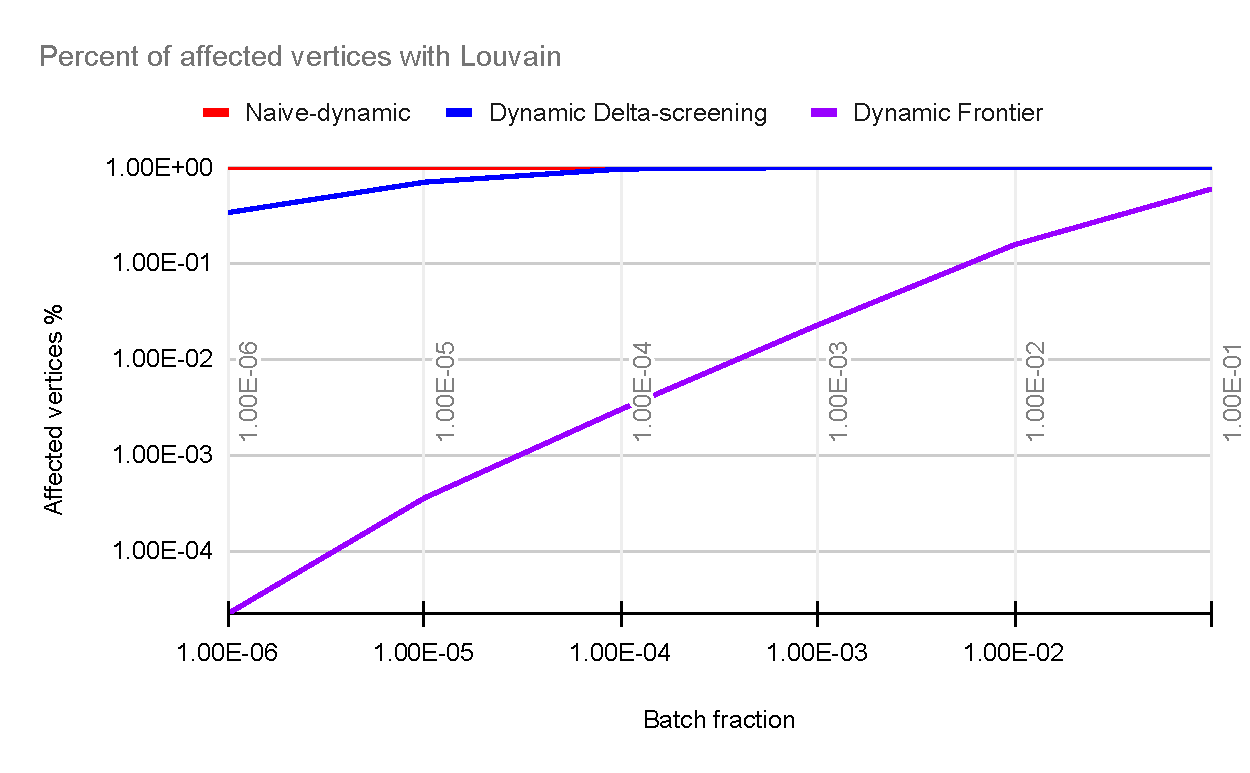
\includegraphics[width=0.48\linewidth]{out/louvain-affected.pdf}
  }
  \subfigure[Dynamic LPA algorithms]{
    \label{fig:louvainrak-affected--rak}
    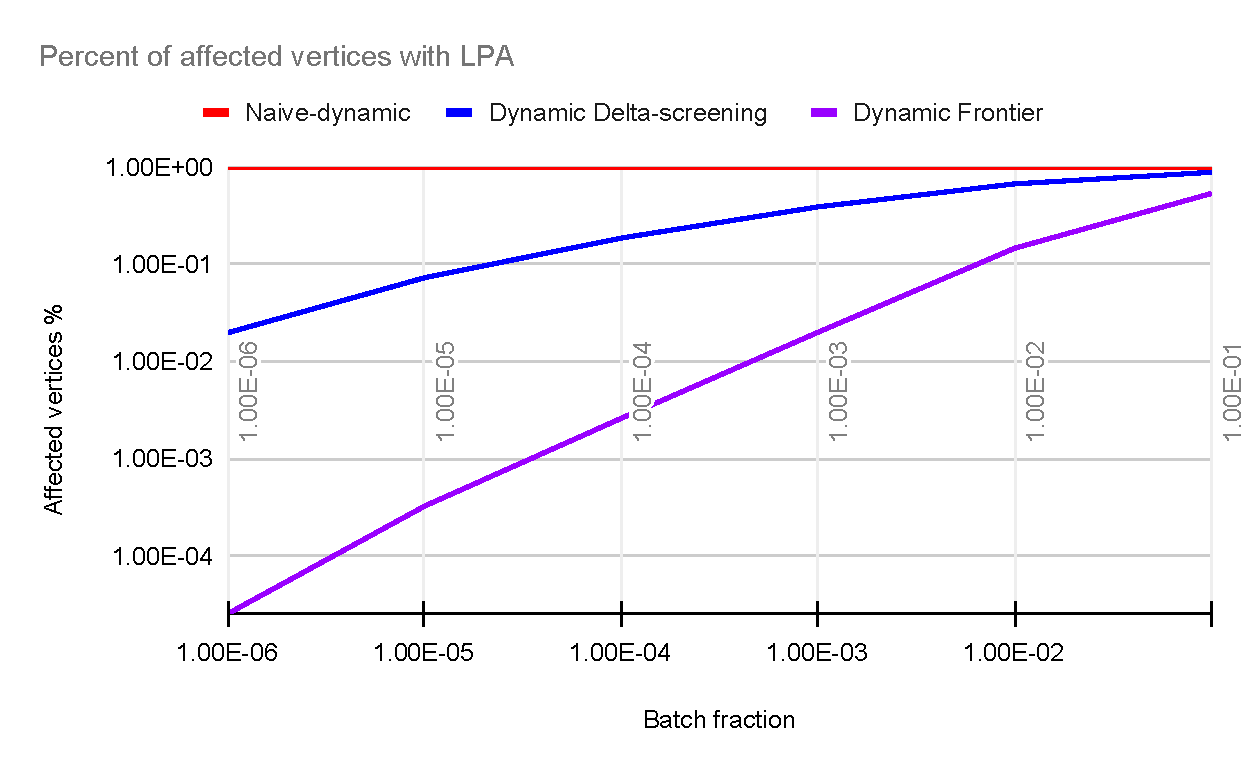
\includegraphics[width=0.48\linewidth]{out/rak-affected.pdf}
  } \\[-2ex]
  \caption{Percent of vertices marked as affected (mean) with \Nai{}, \Del{}, and \Fro{} based \Lou{} and \LPA{}, as mentioned in Sections \ref{sec:louvain-evaluation} and \ref{sec:rak-evaluation}, on graphs in Table \ref{tab:dataset}.}
  \label{fig:louvainrak-affected}
\end{figure*}

\begin{figure*}[hbtp]
  \centering
  \subfigure[Dynamic Louvain algorithms]{
    \label{fig:louvainrak-stability--louvain}
    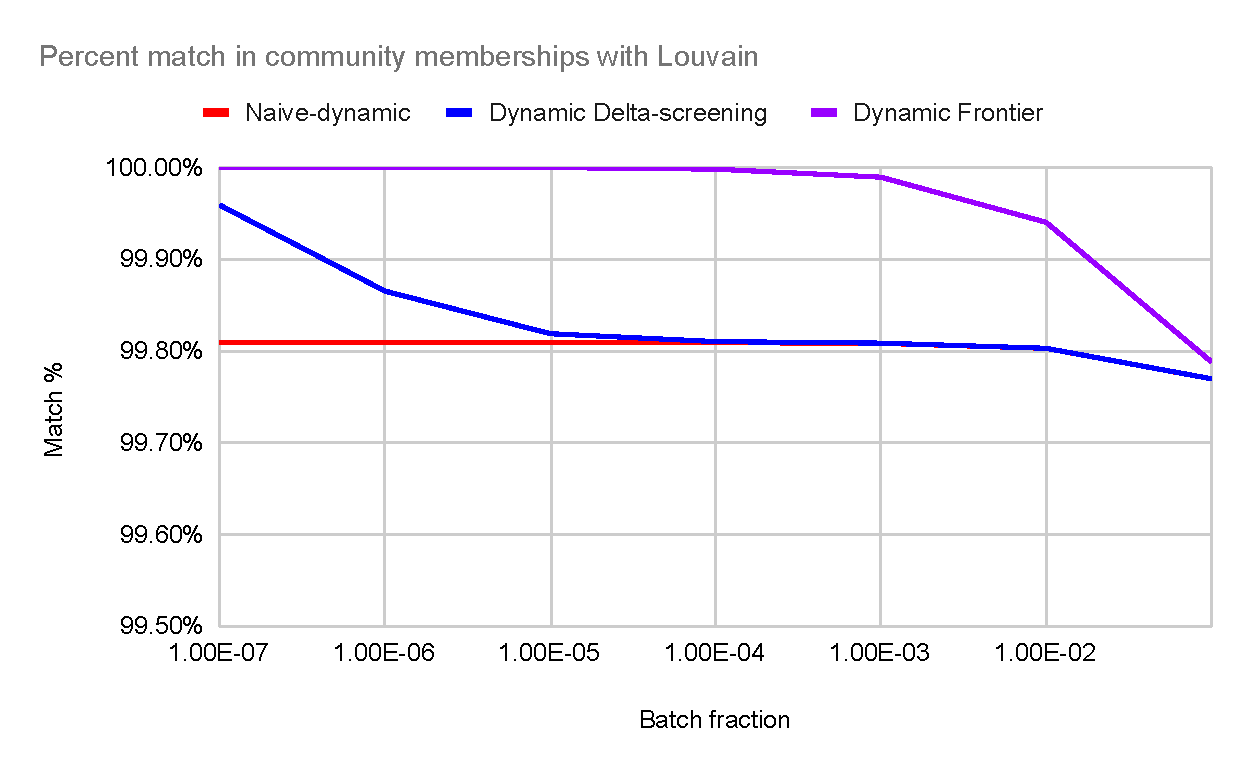
\includegraphics[width=0.48\linewidth]{out/louvain-stability.pdf}
  }
  \subfigure[Dynamic LPA algorithms]{
    \label{fig:louvainrak-stability--rak}
    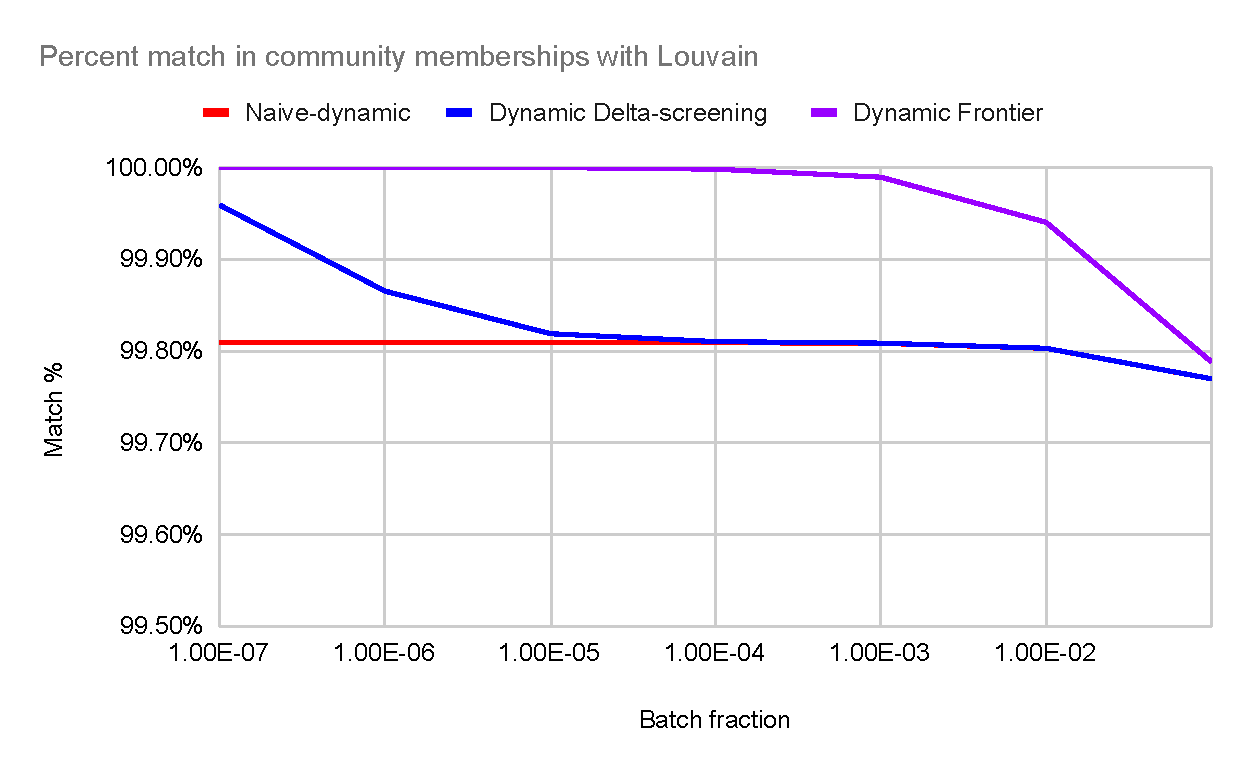
\includegraphics[width=0.48\linewidth]{out/louvain-stability.pdf}
  } \\[-2ex]
  \caption{Percent match in community memberships after reverse and forward batch updates (mean) with \Nai{}, \Del{}, and \Fro{} based \Lou{} and \LPA{}, as mentioned in Sections \ref{sec:louvain-stability} and \ref{sec:rak-stability}, on graphs in Table \ref{tab:dataset}.}
  \label{fig:louvainrak-stability}
\end{figure*}





\subsection{Performance of Dynamic Frontier Louvain (\FroLou{}, Algorithm \ref{alg:louvain})}
\label{sec:louvain-evaluation}

\subsubsection{Overall Performance}

We first study the performance of \FroLou{} on batch updates of size $10^{-7} |E|$ to $0.1 |E|$, and compare it with \StaLou{}, \NaiLou{}, and \DelLou{}. The work of Zarayeneh et al. \cite{com-zarayeneh21} demonstrates improved performance of \textit{$\Delta$-screening} compared to \textit{Dynamo} \cite{com-zhuang19} and \textit{Batch} \cite{com-chong13}. Thus, we limit our comparison to \Del{}. When executing \FroLou{} and \DelLou{}, we reinitialize the community memberships every \verb|RESTART_LOUVAIN| batches with the community labels obtained via \StaLou{} (see Section \ref{sec:restart}). As mentioned in Section \ref{sec:batch-update}, we generate $5$ different random batch updates for each batch size to minimize measurement noise.

Figure \ref{fig:louvain--am} shows the average results of the experiment. We observe the following from Figure \ref{fig:louvain--am}. The modularity of communities obtained by all the dynamic approaches is nearly identical. \FroLou{} converges the fastest with an average speedup of $1.5\times$ over \NaiLou{}. On small batch updates, atomics hinder the speedup. This isn't a reflection of our approach's inefficiency but rather a challenge posed by the parallel implementation of Louvain algorithm. As the batch size increases, the number of vertices marked as affected by \FroLou{} increases. This results in an increase in the time taken by \FroLou{} as the batch size increases. Further, as Figure \ref{fig:louvain--all} shows, dynamic approaches significantly outperform \StaLou{} on \textit{social networks}, \textit{road networks}, and \textit{k-mer protein graphs} (which do not have a dense community structure, or have a low $|E|/|V|$ ratio).

\paragraph{Performance of Dynamic $\Delta$-screening (\DelLou{})}

We note that \DelLou{} does not perform better than \NaiLou{}. This is because it tends to mark a large fraction of the vertices as affected, even for small batch updates. Our experiments on the graphs in Table \ref{tab:dataset} indicate that compared to the \FroLou{}, the \DelLou{} marks nearly $44\times$ more vertices as affected on a batch size of $10^{-3} |E|$.

\paragraph{Slowdown of static algorithm}

Uniform batches of insertions/deletions arbitrarily disrupt the original community structure. This results in \StaLou{} needing more iterations to converge.


\subsubsection{Comparison with respect to Riedy and Bader \cite{com-riedy13}}

Riedy and Bader propose a batch parallel dynamic algorithm for community detection. They compare the run time of their dynamic algorithm to that of a static recomputation. On the graphs \verb|caidaRouterLevel|, \verb|coPapersDBLP|, and \verb|eu-2005|, from \cite{com-riedy13} and at the batch size of $0.1|E|, 0.03|E|,$ and $0.1|E|$ respectively, they report a speedup of $40\times$, $1.08\times$, and $327\times$, respectively, over their corresponding static algorithm performing a full recomputation. On these three graphs and batch sizes, \FroLou{} achieves a speedup of $6.1\times$, $10.9\times$, and $4.2\times$, respectively, compared to a full static recomputation. This might compare unfavorably with the speedups claimed by Riedy and Bader \cite{com-riedy13}. However, note from Section \ref{sec:introduction} that the algorithm of Riedy and Bader \cite{com-riedy13} does not identify cascading changes to communities. In addition, as their source code is not available, we could not do a more direct comparison.


\subsubsection{Stability}
\label{sec:louvain-stability}

Intuitively, if the graphs $G^t$ and $G^{t'}$ are identical for some $t$ and $t'$, we expect \FroLou{} to produce the same communities for $G^t$ and $G^{t'}$. We refer to this property of a dynamic algorithm as its stability, measured as the percentage of vertices that agree on the community label across two identical graphs. Vertices within weak community structures tend to be unstable, as they may connect to multiple communities with similar strength.

To measure the stability of \NaiLou{}, \DelLou{}, and \FroLou{}, we proceed as follows. Let $G$ be an initial graph. We generate random batch updates of size $10^{-7} |E|$ to $0.1 |E|$ consisting of edge deletions to obtain the graph $G^1$. We then apply each of the above algorithms on $G^1$ to identify the new communities. Subsequently, we create another batch of updates that consists of inserting the edges deleted in the prior time step. This graph, $G^2$, is essentially the original graph $G$. We obtain the community labels of the vertices in the graph $G^2$ by appealing to the dynamic algorithms. Finally, we compare the community label of each vertex in the graphs $G$ and $G^2$. The resulting match in community membership of vertices with \NaiLou{}, \DelLou{}, and \FroLou{} on batch updates of size $10^{-7} |E|$ to $0.1 |E|$ is shown in Figure \ref{fig:louvainrak-stability--louvain}.

From Figure \ref{fig:louvainrak-stability--louvain}, we observe that\NaiLou{} and \DelLou{} have minimum of $99.68\%$ match with the original community memberships across all batch sizes, while \FroLou{} has a minimum of $99.70\%$ match. This indicates that all these algorithms are stable.




\subsection{Performance of Dynamic Frontier LPA (\FroLPA{}, Algorithm \ref{alg:rak})}
\label{sec:rak-evaluation}

\subsubsection{Overall Performance}

In this experiment, we study the performance of \FroLPA{} with batch updates of size ranging from $10^{-7} |E|$ to $0.1 |E|$, and compare it to \StaLPA{}, \NaiLPA{}, and \DelLPA{}. Unlike \Lou{}, none of the \LPA{} based dynamic approaches require re-initialization of communities every \verb|RESTART_LOUVAIN| batches. As discussed in Section \ref{sec:batch-update}, we employ $5$ distinct random batch updates for every batch size in order to minimize measurement noise.

Figure \ref{fig:rak--am} shows the average result of the experiment. While all approaches obtain communities of equivalent modularity, \FroLPA{} converges on average $10.0\times$ faster than \NaiLPA{} from a batch size of $10^{-7} |E|$ up to $0.01 |E|$. As shown in Figure \ref{fig:rak--all}, it has good performance on \textit{web graphs} and \textit{social networks} (graphs with high $|E|/|V|$ ratio). Note, however, that the quality of communities obtained with \LPA{} is not on par with \Lou{}.

\paragraph{Performance of Dynamic $\Delta$-screening}

Further, we note that \DelLPA{} generally fails to perform better than \NaiLPA{}. This is because it tends to mark a large fraction of the vertices as affected (see Figure \ref{fig:louvainrak-affected--rak}), and has a high associated overhead.

\paragraph{Slowdown of static algorithm}

As mentioned in Section \ref{sec:louvain-evaluation}, the uniform batches of insertions/deletions arbitrarily disrupt the original community structure, necessitating more iterations for \StaLPA{} to converge.


\subsubsection{Stability}
\label{sec:rak-stability}

Just as in Section \ref{sec:louvain-stability}, we study the stability of \NaiLPA{}, \DelLPA{}, and \FroLPA{} on random batch updates of size $10^{-7} |E|$ to $0.1 |E|$. From the results, shown in Figure \ref{fig:louvainrak-stability--rak}, we observe that \NaiLPA{} and \DelLPA{} have minimum of $95.53\%$ match with the original community memberships across all batch sizes, while \FroLPA{} has a minimum of $95.75\%$ match. This indicates that \FroLPA{} is stable.




\subsection{Performance of Dynamic Frontier Hybrid Louvain-LPA (\FroHyb{}, Algorithm \ref{alg:hybrid})}
\label{sec:hybrid-evaluation}

\subsubsection{Overall Performance}

We now study the performance of \FroHyb{}, which uses \StaLou{} every \verb|RESTART_HYBRID| batches and uses \FroLPA{} for updating communities for the remainder batches (see Sections \ref{sec:dynamic-hybrid} and \ref{sec:restart}). We do this on batch updates of size $10^{-7} |E|$ to $0.1 |E|$, and compare it with \FroLou{} and \FroLPA{} (Algorithms \ref{alg:louvain} and \ref{alg:rak}). As stated in Section \ref{sec:batch-update}, we employ five distinct random batch updates for every batch size to minimize measurement noise.

The average modularity of communities obtained by \FroHyb{} is nearly identical to that obtained by \FroLou{}, as shown in Figure \ref{fig:hybrid--am}, while obtaining a mean speedup of $7.5\times$ across batch sizes of $10^{-7} |E|$ to $0.1 |E|$. \FroHyb{} is thus an efficient and high-quality dynamic community detection approach, especially of \textit{web graphs}, as shown in Figure \ref{fig:hybrid--all}, where it significantly outperforms \FroLou{} for smaller batch updates. Note that \FroLPA{} has about the same performance, but obtains communities of lower quality.


\subsubsection{Scalability}
\label{sec:evaluation--hybridss}

Finally, we study the strong-scaling behavior of \FroHyb{} (Algorithm \ref{alg:hybrid}), and compare it with \FroLou{} and \FroLPA{} (Algorithms \ref{alg:louvain} and \ref{alg:rak}). To do this, we fix the batch size at $10^{-3} |E|$, vary the number of threads in use from $1$ to $64$, and measure the speedup of each algorithm to its sequential version. Figure \ref{fig:hybridss} demonstrates scalability of dynamic algorithms with varying thread count, measured as the time taken by the algorithm compared to the same algorithm running on one thread. Again, as indicated in Section \ref{sec:batch-update}, we employ five distinct random batch updates for each batch size to minimize measurement noise.

As shown in Figure \ref{fig:hybridss--am}, \FroLou{}, \FroLPA{}, and \FroHyb{} obtain a speedup of $5.2\times$, $8.7\times$, and $9.6\times$ respectively at $64$ threads; with their speedup increasing at a mean rate of $1.31\times$, $1.44\times$, and $1.46\times$ respectively for every doubling of threads. Also note from Figure \ref{fig:hybridss--all} that \FroHyb{} offers good speedup on \textit{web graphs} and \textit{social networks}, but does not scale well on \textit{road networks} and \textit{k-mer protein graphs} (which have a low $|E|/|V|$ ratio).




%% - https://www.reddit.com/r/intel/comments/l1kut0/what_are_some_of_the_cons_of_hyperthreading/
